\section{Objetivos}


\clearpage
\section{Metodologia}

\begin{table}[htb]
\renewcommand{\arraystretch}{1.3}
\caption{Dados experimentais do equilíbrio líquido-vapor da mistura
etano(1)/propeno(2) a 100 ºF.}
\sisetup{table-format=2.3,round-mode=places,round-precision=3}
\footnotesize
\center
\begin{tabular}{SSS}
\toprule

\midrule 
 {Densidade a 15$^\circ$C, (kg/m$^3$)}		&	{}				&	{858,9}	\\
 {$^\circ$API}								&	{}				&	{33,2}	\\
 {Bbl/mt}									&	{}				&	{7,336}	\\
 {Acidez (mg KOH/g)}						&	{}				&	{0,54}	\\
 {Enxofre (wt\%)}							&	{}				&	{0,249}	\\
 {Sulfeto de Hidrogênio (mg/kg)}			&	{}				&	{1}		\\
 {Enxofre de mercaptanos (mg/kg)}			&	{}				&	{3	}	\\
 {Viscosidade (cSt)} 						&	{10 $^\circ$C}	&	{19,3}	\\
 { }				 						&	{50 $^\circ$C}	&	{5,4}	\\
 {Pour Point ($^\circ$C)}					&	{}				&	{-6}	\\
 {Nitrogênio total (massa\%)}				&	{}				&	{0,142}	\\
 {Wax (massa\%)}							&	{}				&	{-}		\\
 {Wax Appearance Temperature  ($^\circ$C)}	&	{}				&	{-}		\\
 {RVP a 37,8 $^\circ$C (kPa)}				&	{}				&	{26}	\\
 {Umidade (vol\%)}							&	{}				&	{-}		\\
 {NaCl (mg/kg)}								&	{}				&	{-}		\\
 {Níquel (mg/kg)}							&	{}				&	{7,7}	\\
 {Vanádio (mg/kg)}							&	{}				&	{1,9}	\\
 {Ferro (mg/kg)}								&	{}				&	{-}		\\
 {Mercúrio ($\mu$g/kg)}						&	{}				&	{-}		\\
	
\bottomrule
\multicolumn{3}{c}{Fonte: adaptado de \citeonline{TOTSA2016}}
\end{tabular}
\label{tab:tbp}
\end{table}
\clearpage

\begin{table}[htb]
\renewcommand{\arraystretch}{1.3}
\caption{Dados experimentais do equilíbrio líquido-vapor da mistura
etano(1)/propeno(2) a 100 ºF.}
\sisetup{table-format=2.2,round-mode=places,round-precision=2}
\footnotesize
\center
\begin{tabular}{S[table-format=3.0,round-mode=places,round-precision=0]SS|S[table-format=3.0,round-mode=places,round-precision=0]SS}
\toprule
   {T} & {\%. vap.} & {\% vap.}&{T} &
   {\% vap.} & {\% vap.}\\
   {($^\circ$C)} & {(massa)} & {(vol.)}&{($^\circ$C)} &
   {(massa)} & {(vol.)}\\
\midrule 
80  &4.88  &6.60&  340 & 49.61 &53.57\\
90  &5.83  &7.73&  360 & 53.30 &57.18\\
100 &7.01  &9.10&  380 & 56.86 &60.64\\
120 &10.02 &12.54& 400 & 60.31 &63.96\\
140 &13.62 &16.56& 420 & 63.66 &67.16\\
160 &17.05 &20.31& 440 & 66.91 &70.25\\
180 &19.98 &23.47& 460 & 70.06 &73.22\\
200 &22.86 &26.52& 480 & 73.09 &76.05\\
220 &26.08 &29.90& 500 & 75.99 &78.75\\
240 &29.72 &33.65& 520 & 78.73 &81.28\\
260 &33.64 &37.67& 540 & 81.30 &83.64\\
280 &37.71 &41.78& 560 & 83.68 &85.81\\
300 &41.78 &45.85& 580 & 85.87 &87.80\\
320 &45.76 &49.80&     &       &     \\
\bottomrule
\multicolumn{6}{c}{Fonte: adaptado de \citeonline{TOTSA2016}}
\end{tabular}
\label{tab:tbp}
\end{table}
\clearpage

\clearpage
\section{Resultados} 

\begin{figure}[htb]
\centering
{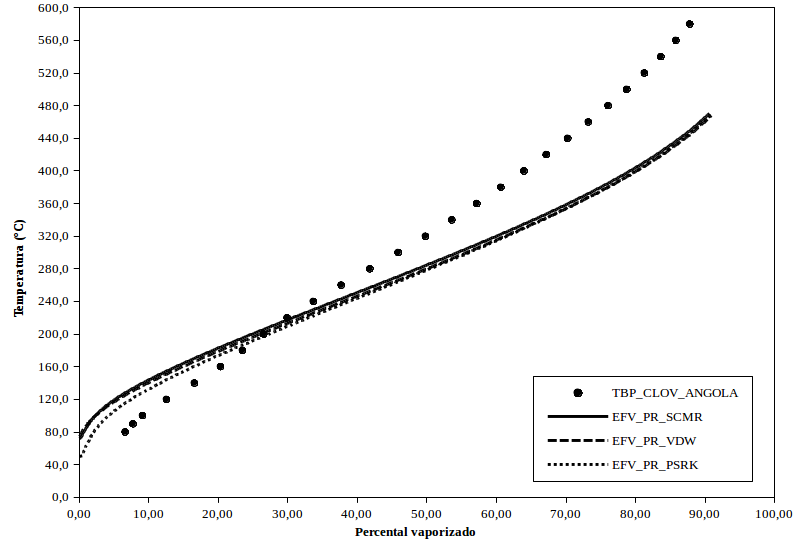
\includegraphics[width=0.8\textwidth]{img/efv.png}} 
\caption{BLA BLA BLA BLA BLA BLA}
\label{fig:efv}
\end{figure} 

\clearpage
\section{Conclusões} 

